\documentclass{article}
\usepackage{graphicx}
\usepackage{amsmath}
\usepackage{array}
\usepackage[font=small, labelfont={sf,bf}, margin=1cm]{caption}
\usepackage{tabularx}
\usepackage{amssymb}


\date{Due: Oct 18  Edit: \today}
\title{ME 200 Homework 7}
\author{James Liu}

\begin{document}
\maketitle
\begin{itemize}
    \item [1.] 
    \begin{itemize}
        \item [a)]     
        \begin{align*}
            \eta = \frac{750-300}{750} = 0.6 = 60\%
        \end{align*}
        \item [b)]
        \begin{align*}
            Q_{12}-W_{12} &= m(u_2-u_1) = 0 (\text{As Ideal gas})\\
            Q_{12}=W_{12} &= 60\text{ kJ}\\
            W_{12} = \int_{V_1}^{V_2} p \text{d}V &= \int_{V_1}^{V_2} \frac{mRT_H}{V} \, dV = mRT_H \ln \left( \frac{V_2}{V_1} \right) = 60 \, \text{kJ}\\
            \ln \left( \frac{V_2}{V_1} \right) &= \frac{60}{2 \times \frac{8.314}{28.97} \times 750}= 0.1394 \text{ m}^3
            \\ V_1 &= 0.348\\
            pv &=nRT\\
            p_1 &= 1237 \text{ kPa} 
        \end{align*}
        \item [c)]
        \begin{align*}
            Q_{12}=W_{12} &= 60\text{ kJ}\\
            Q_{23}&=0\\
            W_{23}=2\times (551.99-214.07)&=676 \text{ kJ}\\
            Q_{34}=W_{34}=60\times \frac{300}{750} &= 24 \text{kJ}\\
            Q_{41}&=0\\
            W_{41}=-W_23=&-676 \text{{kJ}}
        \end{align*}
        \item [d)] \ 
        \begin{figure}[h]
            \centering
            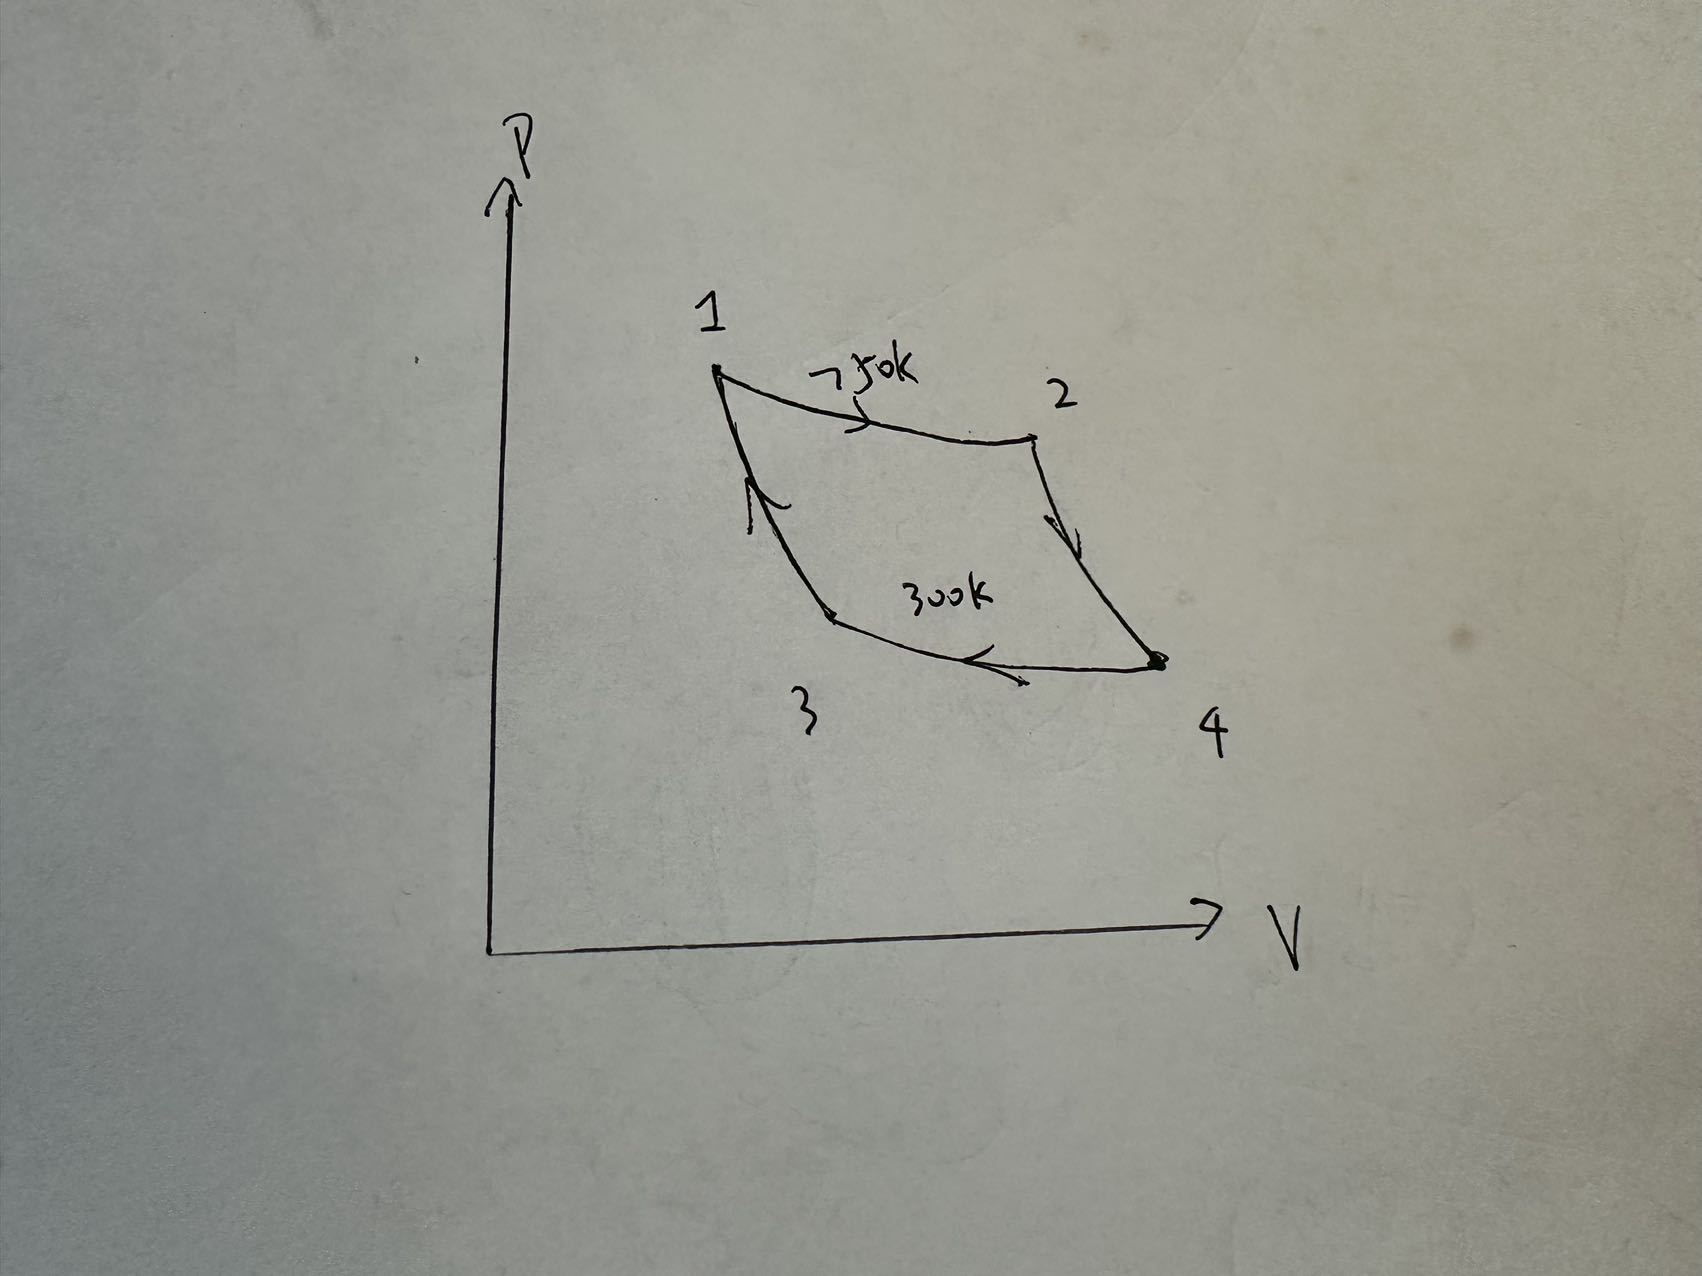
\includegraphics[scale=0.1]{fig/me200-hw6-fig1}
        \end{figure}
    \end{itemize}
    \newpage
    \item [2.]
    \begin{align*}
        h_2=h_f&=1341.96\\
        s_2=s_f&=3.2139\\
        h_3=h_g&=2769.32\\
        s_1=s_2,&\ s_3=s_4\\
        h_4=h_f+xh_g&=105.005+0.652\times 2442.845\\
        &=1697.74\\
        s_2 = s_1 &= s_f+xf_g\\
        3.2139&=0.3671+x\times 8.1926\\
        x&=0.3475\\
        h_1 &= h_f+xh_g\\
        &=953.8553\\
    \end{align*}
    Apply those numbers that were just calculated, we get:
    \begin{align*}
        Q_{12}&=0\\
        W_{12}&=h_2-h_1=388.105\\
        Q_{23}&=h_3-h_2=1427.41\\
        W_{23}&=0\\
        Q_{34}&=0\\
        W_{34}&=h_4-h_3=-1071.6\\
        Q_{41}&=h_4-h_1=743.8847\\
        W_{41}&=0
    \end{align*}
\end{itemize}
\end{document}